%% Bemærk:
%%          Resten af rapporten følger en stil hvor indledninger skrives
%%          med \sffamlily-typen. Denne stil bør også følges her.
%%
{\sffamily
I dette sektion vil vi teste den naive løsning. ved at se om den sortere
de rigtige regioner væk og om løsningen opføre sig på samme måde som vi
har håbet på. Det vil vi gøre ved ført at se på nogle fabrikeret test
billeder, får at se om den naive løsning virker efter meningen og
bagefter vil vi teste på malerierne for at se om den naive løsning kan
bruges i praktisk.
}
  
\subsection{Afprøvning på testbilleder}
Vi vil teste på de samme testbilleder som i sideste afsnit, samt et nyt
testbilleder som blev brugt i forklaringen af den naive metodes, de fire
billeder som vi har valt at test kan se i afsnit \ref{region_detektor} og billedet 
\ref{naiv_masse_original} hvor en grån kasse rundt om en region, betyder
at den er valt til at ligge i det gyldne snit af den naive metode. 

Det første billedet \ref{naiv_blob1}, har fem
regioner og hvor tre af dem blev fundet af reginon detektoren, vores naive
løsning har så sorteret baggrundens regionen og den øverste region i
snitte vær, da de begge krydser marginer og derfor ikke overholder definition
\ref{} . 

\begin{figure}[!h]
	\begin{center}
        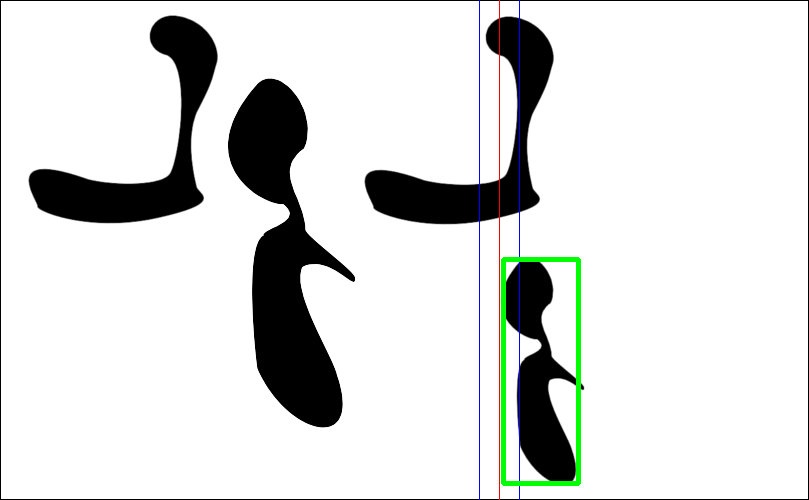
\includegraphics[angle=0,width=0.55\textwidth]{afsnit/afprovning/billeder/naive_losning/naiv_blob1.png}
	\end{center}       
	\caption{Naive algoritme finder en ud af fem regioner}	
	\label{naiv_blob1}
\end{figure}

Det andet billedet \ref{naiv_blob2}, er alle blevet sorteret vær, også
den lille, da den er for lille, derfor ikke overholder definition
\ref{def_interessant} b. 

\begin{figure}[!h]
	\begin{center}
       	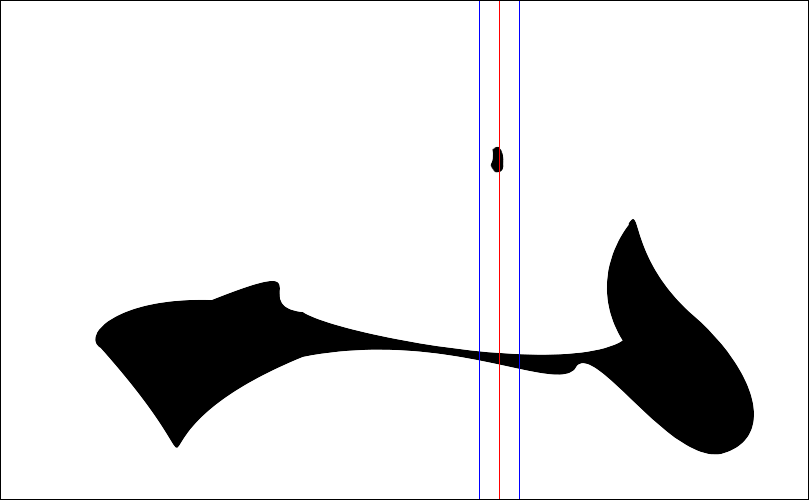
\includegraphics[angle=0,width=0.55\textwidth]{afsnit/afprovning/billeder/naive_losning/naiv_blob2.png}
	\end{center}
	\caption{Værgen den lille region eller den store er fundet} 
   	\label{naiv_blob2}
\end{figure}

I test billedet \ref{naive_hoisont1}, sortere algoritmen
himlen fra, da den krydser margin lidt, men tager jorden med. 

\begin{figure}[!h]
	\begin{center}
       	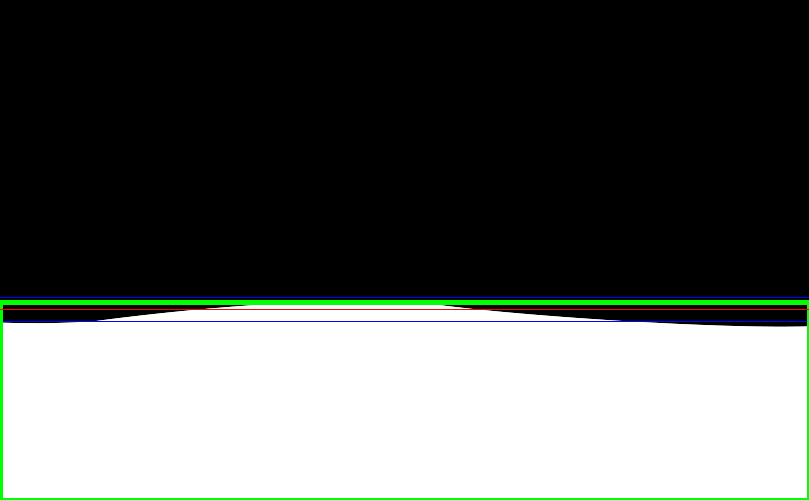
\includegraphics[angle=0,width=0.55\textwidth]{afsnit/afprovning/billeder/naive_losning/naiv_hoisont1.png}
	\end{center}
	\caption{Kun den nederste højrisondt er fundet} 
   	\label{naive_hoisont1}
\end{figure}

\clearpage

\subsection{Afprøvning på malerier}
Vi afprøver den naive algoritme på 6 malerier, først på 3 malerier, hvor regions detektoren virker
efter vores hensigt og så på 3 malerier, hvor region detektoren ikke
virker. Beskrivelsen af hvad der sker i billedet vil står i caption


\begin{figure}[h!!]
	\begin{center}
		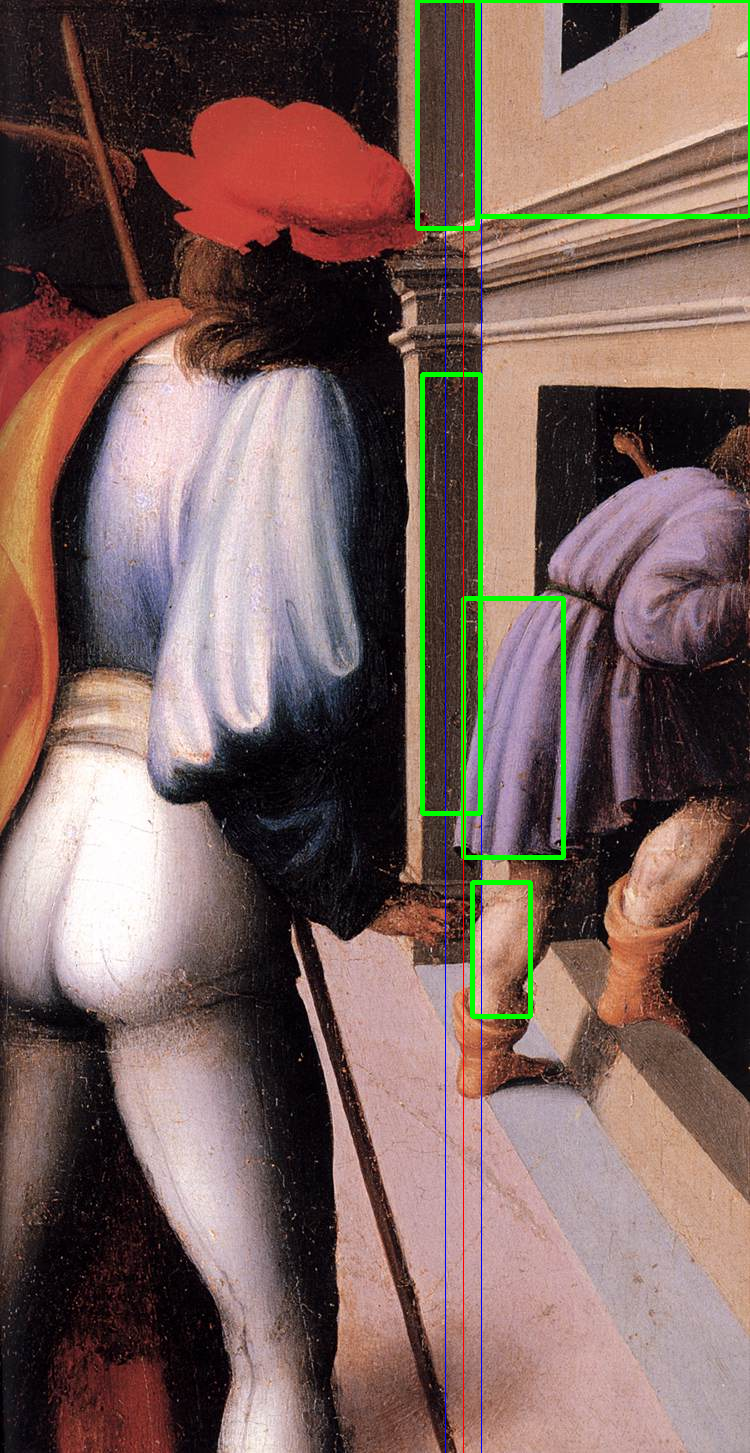
\includegraphics[scale=0.3,angle=0]{afsnit/afprovning/billeder/naive_losning/naiv_kfarver_sdetaljer.png}
	\end{center}
	\caption[]{5 ud af de 6 store regioner fra figur \ref{GRD_virker1} valt til at ligge i snittet, skoene er få små til at blive taget i betragtning}
	\label{naiv_kfarver_sdetaljer}
\end{figure}

\begin{figure}[h!!]
	\begin{center}
		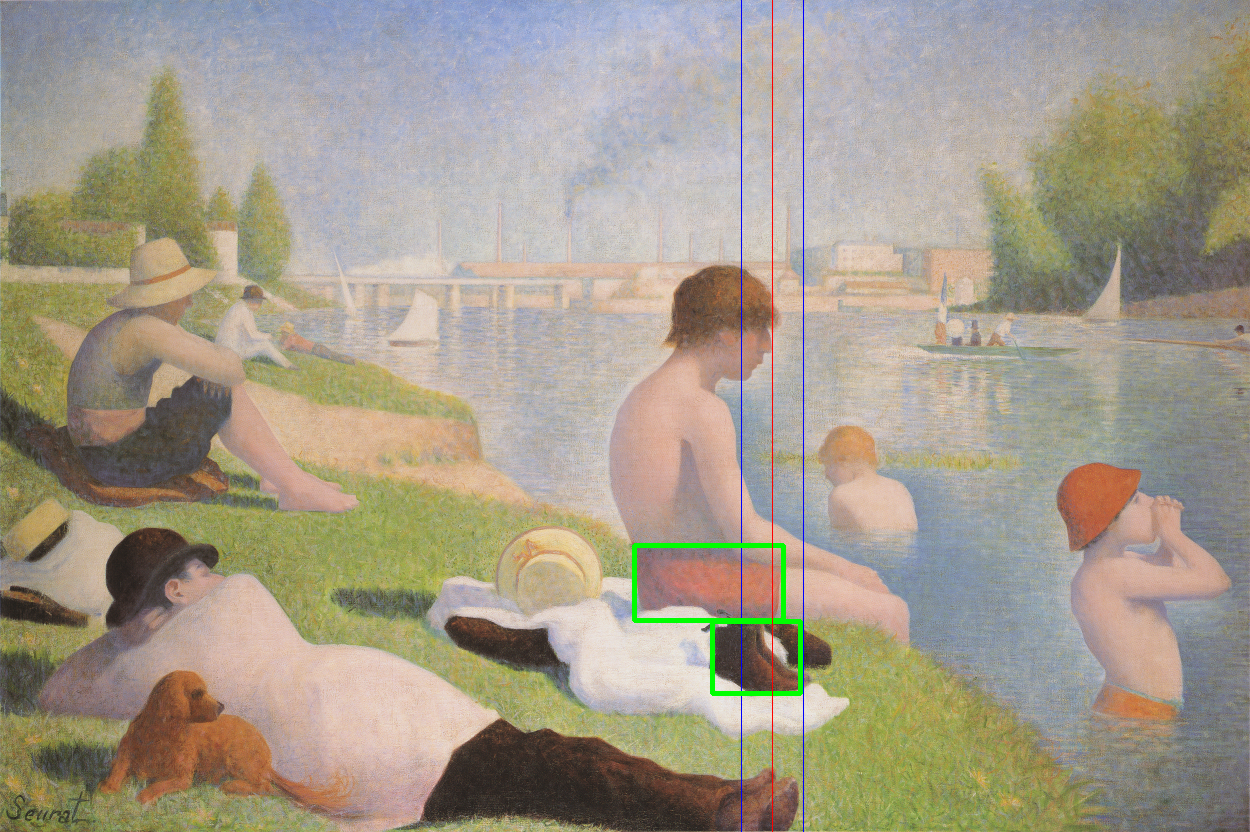
\includegraphics[scale=0.3,angle=0]{afsnit/afprovning/billeder/naive_losning/naiv_mfarver_mdetaljer.png}
	\end{center}
	\caption[]{Bukserne og skoene er tager med af den naive løsning, men drengen er sorteret væk da har krydser snittet}
	\label{naiv_mfarver_mdetaljer}
\end{figure}

\begin{figure}[h!!]
	\begin{center}
		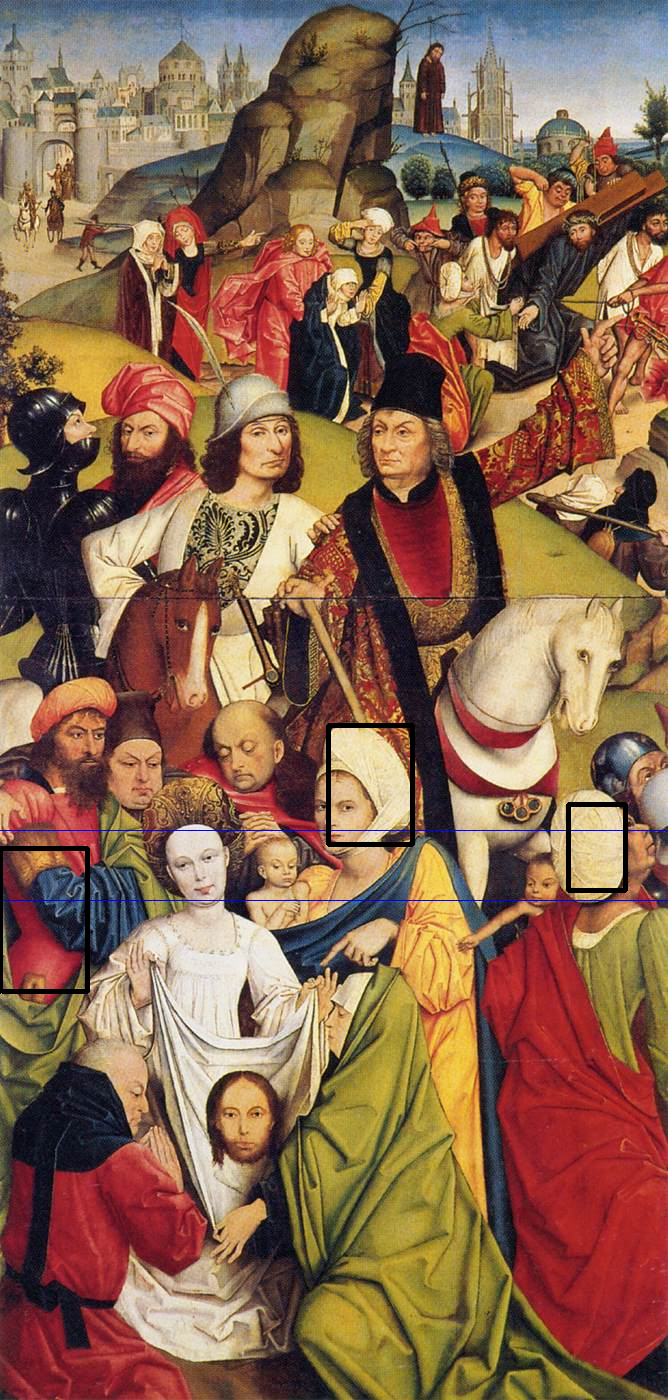
\includegraphics[scale=0.3,angle=0]{afsnit/afprovning/billeder/naive_losning/naiv_kfarver_kdetaljer.png}
	\end{center}
	\caption[]{Et billedet med mange hoder i snittet, hvor 2 af dem bliver godtaget af den naive metode til at ligger i snittet, en trøje bliver desværre også taget med. Navn: Christ Carrying the Cross. År: 1480. Af: Bosch Hieronymus}
	\label{naiv_kfarver_kdetaljer}
\end{figure}

\begin{figure}[h!!]
	\begin{center}
		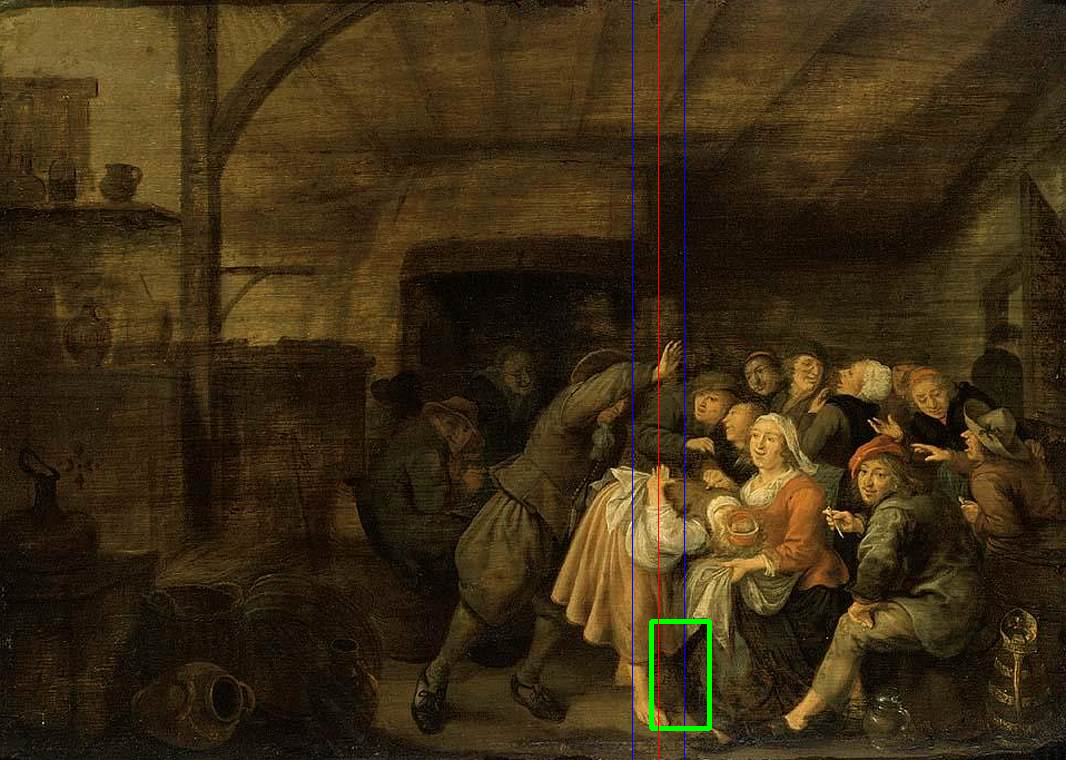
\includegraphics[scale=0.3,angle=0]{afsnit/afprovning/billeder/naive_losning/naiv_virker_ikke1.png}
	\end{center}
	\caption[]{Mallerie hvor region detektor ikke virker, den naive løsning godtager tager en region som ligger helt forkert. Navn: Peasants in an Inn Playing "La Main Chaude". År: Ukendt. Af: Molenaer, Jan Miense.}
	\label{naiv_virker_ikke1}
\end{figure}

\begin{figure}[h!!]
	\begin{center}
		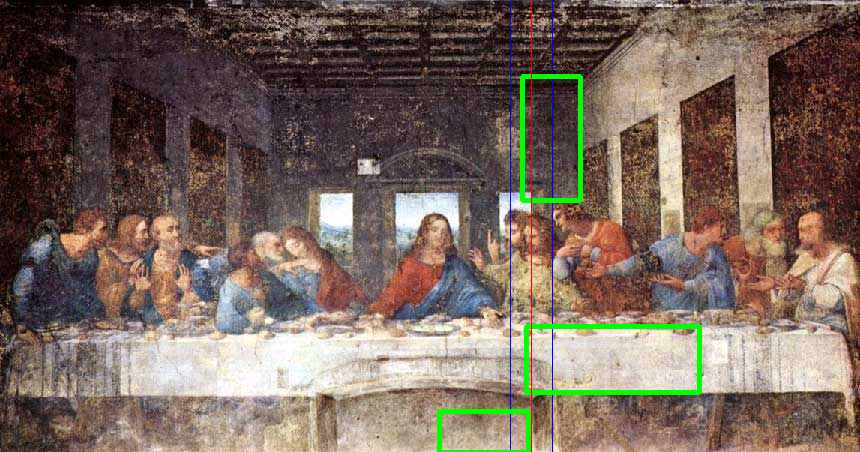
\includegraphics[scale=0.3,angle=0]{afsnit/afprovning/billeder/naive_losning/naiv_virker_ikke2.png}
	\end{center}
	\caption[]{3 regioner bliver godtaget, selv om de ikke er særlige intresante }
	\label{naiv_virker_ikke2}
\end{figure}

\begin{figure}[h!!]
	\begin{center}
		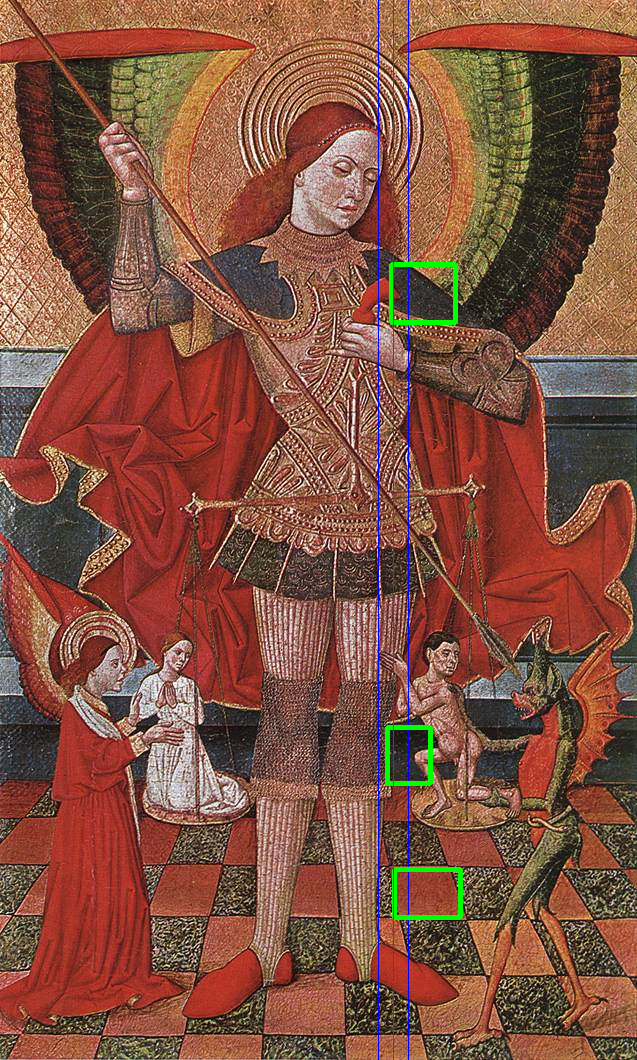
\includegraphics[scale=0.3,angle=0]{afsnit/afprovning/billeder/naive_losning/naiv_virker_ikke3.png}
	\end{center}
	\caption[]{Der bliver fundet 3 region, hvor kun en af dem passer på en ting i billedet}
	\label{naiv_virker_ikke3}
\end{figure}
\clearpage

\subsection{Konkulution}
Det virker som om den naive løsning virker efter vores entationer dog
med nogle få falske positive, hvis region detektoren virker på
malerierne, dog fejler den på malerier hvor region detektoren fejler, og
kommer med en masse falske positive.
